\begin{figure}[t]
\centering
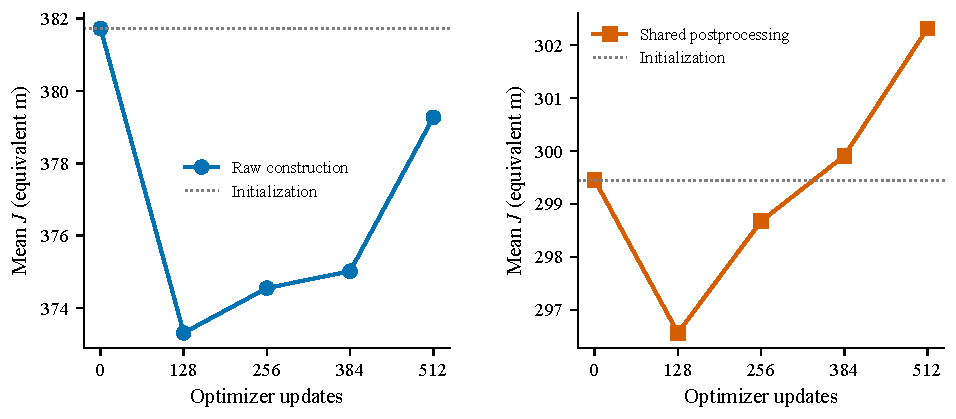
\includegraphics[width=0.95\textwidth]{rc3_constructive/figures/learning_curve.pdf}
\caption{One-seed constructive REINFORCE pilot on 48 model-selection scenes. Raw and uniformly postprocessed costs $J=L+0.75K$, in equivalent meters, are shown separately. The dotted lines mark initialization. These are model-selection results, not independent test or cross-seed evidence.}
\label{fig:constructive-learning}
\end{figure}

\begin{figure}[t]
\centering
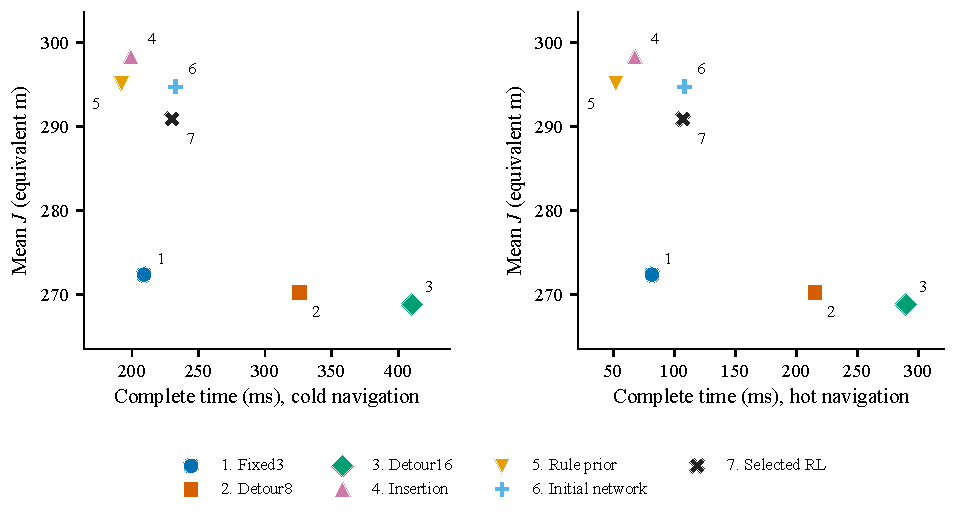
\includegraphics[width=0.95\textwidth]{rc3_constructive/figures/quality_time.pdf}
\caption{Cost--time screening on 24 development scenes, with two interleaved repetitions per method and cache condition. Repetitions are averaged within scenes before taking the time median. Mean $J=L+0.75K$ and median complete time are marginal summaries. CPU single-thread time includes input preparation through final validation; model loading and separately recorded raw-plan research audits are excluded.}
\label{fig:constructive-quality-time}
\end{figure}
